\documentclass[12pt]{article}
\usepackage{url}
\usepackage[left=1.1 in, right=1.1 in, top=1.1 in, bottom = 1.1in]{geometry}
\usepackage{amsmath}
\usepackage{graphicx}
\usepackage{comment}
\usepackage[dvipsnames]{xcolor}

\begin{document}

% \begin{titlepage}
% \begin{flushleft}
% \today \\\hspace{\fill}\\
% Statement of Work, RIPS 2019\\
% Gaming Graphics Artifacts Detection Using Deep Learning Algorithms\\\hspace{\fill}\\
% Advanced Micro Devices\\\hspace{\fill}\\
% Nicholas Malaya, Ph.D.\\
% Max Kiehn, AMD Fellow\\
% Alan Lee, AMD CVP\\\hspace{\fill}\\
% Dear Industry Sponsors,\\\hspace{\fill}\\

% Please find the Statement of Work for the AMD RIPS 2019 project attached. This document is intended to address the definition of the proposed project, our approaches to its completion and a tentative schedule of our progress reports.\\\hspace{\fill}\\
% Sincerely,\\\hspace{\fill}
% \end{flushleft}
% \begin{flushleft}
% RIPS Academic Mentor:\qquad\qquad  Project Manager:\\
% Dr. Shantanu Joshi \qquad\qquad  \quad $\>\>$ Parmida Davarmanesh \\ \hspace{\fill}\\\\
% Student Participants:\\
% Parmida Davarmanesh,\\
% Kuanhao Jiang,\\
% Tingting Ou,\\
% Artem Vysogorets\\
% \end{flushleft}



% \end{titlepage}
% \tableofcontents



% \newpage

\begin{titlepage}
    \begin{center}
        \vspace*{1cm}
 
        \Huge
        \textbf{Statement of Work\\RIPS 2019 Team AMD}
 
        \vspace{2cm}
        
        Gaming Graphics Artifact Detection Using Deep Learning Algorithms\\
        
        \vspace{2cm}
        
        \begin{flushleft}
        \small
        \textbf{Paticipating Students: \qquad \qquad\qquad \qquad \qquad \qquad \qquad \qquad  Industry Mentors:\\}
            Parmida Davarmanesh\qquad \qquad \qquad \qquad \qquad \qquad \qquad \qquad \qquad \qquad Nicholas Malaya, Ph.D.\\
            Kuanhao Jiang \qquad \qquad\qquad\qquad \qquad \qquad \qquad \qquad \qquad \qquad \qquad$\>\>\>$ Max Kiehn, AMD Fellow\\
            Tingting Ou \qquad \qquad\qquad\qquad\qquad\qquad \qquad \qquad \qquad \qquad \qquad \quad $\>\>\>\>$ Alan Lee, AMD CVP \\
            Artem Vysogorets  \qquad \qquad\qquad\qquad\qquad\qquad \qquad \quad \qquad \qquad \qquad $\>\>$ \textbf{Academic Mentor:\\}
        \qquad \qquad\qquad\qquad \qquad \qquad \qquad \qquad \qquad  \qquad \qquad \qquad \qquad \qquad \qquad   Dr. Shantanu Joshi\\
        \end{flushleft}
 
 
        

        
 
        \vspace{1.5cm}
 
     
 
        \vfill
 
       
        \includegraphics[width=0.4\textwidth]{ipam.jpeg}
 
        \Large
        07/02/2019
 
    \end{center}
\end{titlepage}


\section{Project Background}
Founded in 1969 as a Silicon valley start-up, Advanced Micro Devices (AMD) is an American company specializing in semiconductor products such as microprocessors, motherboard chipsets and graphic processors. With these products, AMD brings advances in high-performance computing to both IT businesses and consumer markets. In particular, Graphic Processing Units (GPUs) developed and manufactured by AMD empower different modifications of game consoles  including Xbox and PlayStation.\\

\noindent To ensure quality gameplay, it is critical to perform testing of the GPUs and their compatibility with the requirements of each specific video game before these products reach mass market. Given the overwhelming complexity of modern video games, finding graphics glitches is an extremely laborious task that still involves manual validation,  verification, and bug reporting mechanisms. However, failure to do so might lead to serious financial and reputational losses. Video game players from all around the world report an overwhelming number of different screen artifacts that negatively affect the gameplay. Some of the most common artifacts include screen-tearing, checkerboard artifacts and flickering (Figure \ref{fig:1}).
\begin{figure}[!ht]
\centering
\includegraphics[scale=0.15]{screen-tearing.jpg}
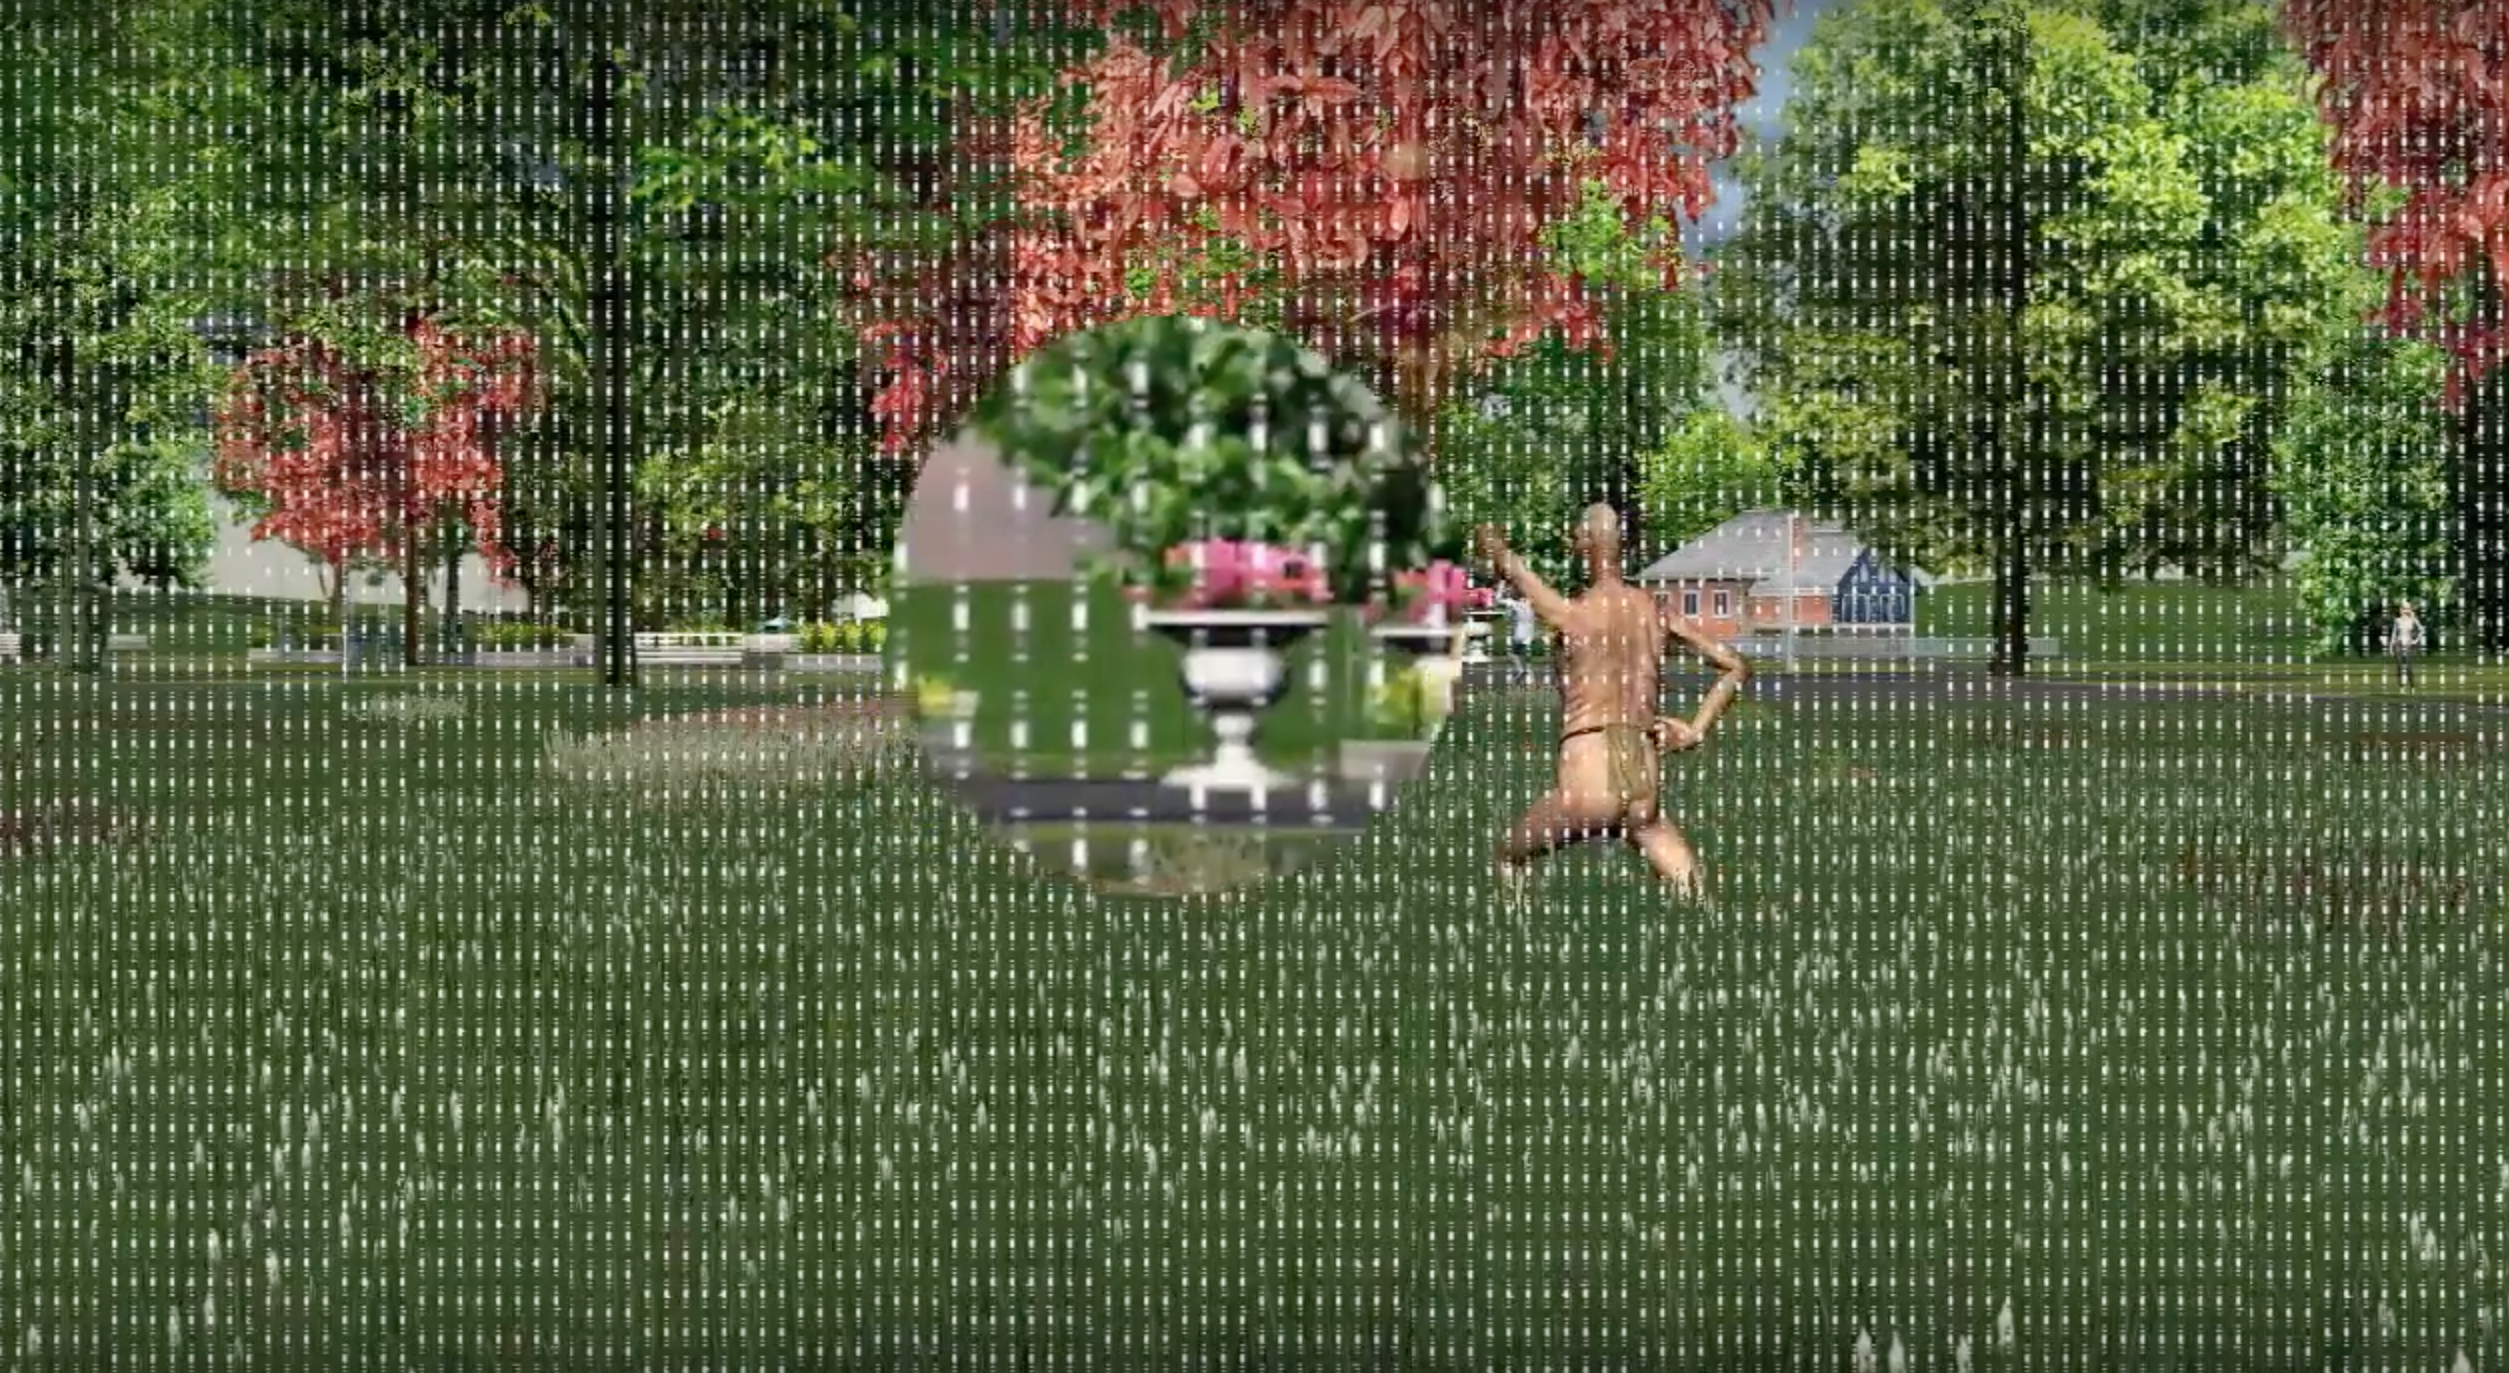
\includegraphics[scale=0.16]{checkered-screen.png}
\caption{Examples of screen-tearing (left) and checkerboard screen artifacts (right).} %Images are borrowed from Chai Wei Ong \cite{Ong} and AMD \cite{AMD}.}
\label{fig:1}
\end{figure}\\


\begin{figure}[!ht]
\centering
\includegraphics[scale=0.19]{bug1.png}
\includegraphics[scale=0.23]{bug2.png}
\includegraphics[scale=0.19]{bug3.png}
\includegraphics[scale=0.15]{distortion.png}
\caption{Other examples of bugs and distortions.}
\label{fig:2}
\end{figure}


%\textcolor{red}{Add other sources of glitches if you have any.}%

\noindent In light of the increasing market share of AMD GPUs \cite{amd}, and the extent to which the gaming industry relies on AMD GPUs, glitch detection is an important problem to be solved.\\\hspace{\fill}\\
Thus, our project, as proposed by AMD, is aimed at developing deep learning models for automated detection of gaming graphics artifacts (glitches) arising from GPU malfunctions or from software bugs during normal operations of GPUs. Very few automated solutions exist for artifact detection, both while real time gameplay and offline game testing.  An effective solution to this problem  has a tremendous potential for facilitating testing of GPUs and their compatibility with newly developed games. Our proposed solution is outlined in the following sections. 

\section{Objectives}
\noindent There is a great variety in the types and visual appearances of possible artifacts in video games. Artifacts could be caused by software or hardware defects, and depending on the type of the glitch, they might not even be recognizable by inspection of the individual frames. While our ultimate goal is to detect all different kinds of common glitches (anomalies) in gaming images, we will develop several different models step by step, beginning with the simpler ones that may evolve into more  complicated ones in the future. 

\subsection{Main Objective}
Our first objective is to build models that are able to identify frames that only have a certain type of artifact. For example, we may present a model that is able to determine whether frames have screen tearing or not. We may also build another model which is capable of detecting blurred images. After achieving this goal, we will work to come up with a model that will determine if images have other types of  artifacts, and if possible, label them.

\subsection{Additional Objectives}
Time permitting, we will investigate a real-time detection model. The model is expected to detect anomalies efficiently and effectively while the game is being played and data is being collected during a real time operation. Detecting distortions in games (bottom right image in figure \ref{fig:2}) is a more challenging task as it requires a lot of data for the models to learn ``the norm" in a given game. If possible, we will attempt to accomplish this task as well.\\ 

\section{Proposed Approach}

In this section, we will discuss our strategy in acquiring data and present possible approaches and algorithms to be explored during the research.

\subsection{Data}
In the next following subsections, we outline the data generation and preprocessing. 

\subsubsection{Data Generation}
Since AMD gaming artifact data is proprietary and not publicly available, we propose a system to generate and label our own database. To produce normal glitch-free images, we will extract frames from YouTube videos using scene filters. Those videos are screen recordings of people playing video games. Specifically, we will use images from games including but not limited to \textit{Borderlands} -- a first-person shooting game, \textit{Dirt Rally} -- a racing game, and \textit{Civilization 6} -- a turn-based strategy game\ref{fig:games_data}. 

\begin{figure}[!ht]
\centering
\includegraphics[scale=0.08]{gameimage.jpg}
\caption{Images Generated from Gaming Videos of Dirt Rally (left), Civilization 6 (middle) and Borderlands (right)}
\label{fig:games_data}
\end{figure}

% \noindent The specification of the normal dataset is summarized in the following table:
% \begin{center}
%  \begin{tabular}[h!]{|c|c|c|c|} 
%  \hline
% Game Name & %\textcolor{red}{Duration?} Size 
% number of frames & Dimension & Color Channel \\
%     \hline\hline
%     Dirt Rally & 465 & 1920*1088 & RGB \\
%     \hline
%     Civilization & 452 & 1920*1088 & RGB\\
%     \hline
%     Borderlands & 3143 & 1920*1088 & RGB\\
%     \hline
% \end{tabular}
% \end{center}

\noindent Glitched (anomalous) game images, on the other hand, are challenging to find as they are relatively rare. Therefore, we will develop software to synthetically generate glitched images including blurring, screen-tearing, adding checkerboard patterns, etc. 

\subsubsection{Data Preprocessing}

The data images will be scaled down to 224x224 pixels, which is a standard dimension for the purposes of Convolutional Neural Networks. The bilinear interpolation and seam carving are typically employed for this purpose. The final choice between these two scaling operations will be made via training preliminary models.\\\hspace{\fill}\\
\noindent It is likely that additional image transformations might facilitate the extraction of certain types of screen artifacts. For example, due to the visual regularity and periodicity inherent to the ``checkerboad'' screen glitch, it could be better captured by considering frames in frequency domain rather than in spatial domain. In fact, Fourier transforms of signals are successfully used for periodic pattern recognition \cite{russians}. There are plenty of other methods of image regularity extraction, such as convolution, Haar Wavelet transform and Hough transform \cite{transform1, transform2}. We will utilize some of these methods at the preprocessing stage to facilitate learning the ``checkerboard'' screen artifact. We are currently in search of other image transformations that could be beneficial for other types of common glitches (Figure \ref{fig:1}, \ref{fig:2}).





%There are two widely used mathematical techniques that we seek to utilize in our project: Singular Value Decomposition (SVD), and Fourier Transform. These techniques have shown to be very useful in the field of image processing. We will explore these two methods to see whether we can better classify defect images.%


\subsection{Methods}
\subsubsection{Supervised Learning}
With sufficient labelled data, we can train supervised learning models to predict the existence of glitches. One possible extension is to use supervised learning to predict the existence of certain types of glitches.\\

\noindent Since the input data are mostly images, we can use convolutional neural networks (CNNs) to capture the features. We plan to use the prediction of previously established and widely used CNN architectures, LeNet \cite{726791}, as the baseline for our project. Possible extensions to CNN are residual neural networks and inception neural networks \cite{DBLP:journals/corr/HeZRS15, DBLP:journals/corr/SzegedyLJSRAEVR14}, which may yield a higher prediction accuracy by enabling deeper networks.\\

\noindent Another strategy for artifact detection is to monitor the change in consecutive (or nearby) frames in a video game. If we are able to gather enough video recordings of the games, then we can obtain pairs of nearby frames to form new data points. Each data point will include two consecutive frames. For training, a pair is labelled as 0 if the two images are both glitched or non-glitched, and 1 otherwise. In this way, we will have relatively balanced data to train the supervised models and capture the starting or ending point of the glitches. During testing, we continuously feed pairs of nearby frames to the model, and if it outputs 1 as the label, then it is likely that a glitch occurred or disappeared going from the first frame to the second.

\subsubsection{Unsupervised Learning/Semi-supervised Learning}
To identify rare glitches that are not yet identified or are difficult to manually produce, we also employ unsupervised learning algorithms. For instance, CNN-based variational autoencoders in conjunction with principle component analysis can be used to reduce data dimensionality. \\


\noindent Reduced data can be fed to supervised learning algorithms (such as CNN, support vector machine, linear regression, etc.) to make predictions. Moreover, after training an autoencoder, we can remove patches from testing images and then feed the residual patches to the autoencoder. By comparing the residual patches with reconstructed patches the model may be able to detect the existence of anomalous features.\\


\begin{comment}
\textcolor{red}{this is going to be a stretch. Methods using SVDs are generally not directly applied for image artifacts. They will work well for time signal denoising. Images generally require something sophisticated. Either remove this paragraph, or change the formulation. So image denoising  is a separate problem from anomaly detection, and not what we are trying to solve.}
\noindent In addition to the methods mentioned above, we seek to explore a technique that is widely used in image processing: Singular Value Decomposition (SVD). This linear algebra technique can be used to denoise images, and by comparing the denoised image and the original image we might be able to determine whether the original image contains an artifact. 
\end{comment}

\noindent We will also train a generative adversarial network (GAN)\cite{2014arXiv1406.2661G} 
and then use the discriminator to make predictions. Other possible unsupervised learning algorithms that may be considered include one-class support vector machine, Gaussian mixture model, and K-nearest neighbors.


\section{Deliverables}
\begin{itemize}
    \item From the RIPS team to industry sponsors:
    \begin{itemize}
        \item Weekly conference call meetings
        \item Midterm oral presentation
        \item Midterm progress report
        \item Oral presentation at AMD site
        \item Projects Day presentation
        \item Final report of findings
        \item Software used to design models
    \end{itemize}
    \item From Industry Sponsors to the Rips team
    \begin{itemize}
        \item Weekly conference call meetings with Dr. Nicholas Malaya
        
        \item A joint conference call with Dr. Nicholas Malaya and Dr. Max Kiehn during weeks 1-3
        
        \item Project specifications
        
        \item AMD site visit
    \end{itemize}
\end{itemize}

\section{Schedule}
\begin{itemize}
    \item Week 1-3
    \begin{itemize}
         \item Research the subject matter: causes/types of glitches, anomaly detection, GPU details (conference call with Max)
         \item Generate the data
         \item Implement basic CNNs and GANs
    \end{itemize}
    
    \item Week 4-6
    \begin{itemize}
         \item Implement extensions to existing algorithms
         \item Prepare and present midterm written report and oral presentation 
    \end{itemize}
    \item Week 7-9
    \begin{itemize}
        
         \item Implement real-time glitch detection
         \item Perform any further experiments based on results at hand
          \item Site visit
         \item Prepare and present final report
         
         
    \end{itemize}
\end{itemize}

 
 \begin{comment}
 
% \begin{thebibliography}{99}

% \bibitem{AMD} AMD Youtube Channel,
% \textit{AMD Support: How to Troubleshoot Checkerboard Pattern Display Corruption}. Published May 13, 2013. Accessed Jun. 28, 2019.\\
% \url{https://youtu.be/lW1wsI1-U0k}

% \bibitem{russians} Chernov, T. et al.,
% \textit{A method of periodic pattern detection on document images}. Published May, 2015. Accessed Jun. 28, 2019.\\
% \url{http://www.scs-europe.net/dlib/2015/ecms2015acceptedpapers/0506-is_ECMS2015_0111.pdf}

% \bibitem{dr} GameRiot,
% \textit{Dirt Rally Career Mode Gameplay Walkthrough Part 1-3} \\
% \url{https://youtu.be/iR157tmQ_fQ}\\
% \url{https://youtu.be/wS-rQ-egusU}\\
% \url{https://youtu.be/Eko_Whref9M}

% \bibitem{c6} 2BCProductions2BC,
% \textit{Civilization 6 Rome} \\
% \url{https://www.youtube.com/playlist?list=PL5Epq2dfiaU2frvpJuSA_TAvCQg4yaimS}

% \bibitem{bdl} MrBlockzGaming,
% \textit{Borderlands The Pre-Sequel FULL Walkthrough No Commentary Gameplay Part 1 Longplay (PC)} \\
% \url{https://youtu.be/0CFMoTs_gRM}

% \bibitem{Ong} Ong, Chai Wei,
% \textit{Reducing screen tearing and input lag}. Published Jul. 4, 2015. Accessed Jun. 28, 2019.\\
% \url{https://bit.ly/2KItAtC}

% \bibitem{transform1} Ruiz, L. et al,
% \textit{Methods for Automatic Extraction of Regularity Patterns and Its Application to Object-Oriented Image Classification}. Accessed Jul. 1, 2019.\\
% \url{http://www.pf.bgu.tum.de/isprs/pia07/puba/PIA07_Ruiz_et_al.pdf}

% \bibitem{transform2} Asha, V. et al,
% \textit{Periodicity Extraction using Superposition of Distance Matching Function and One-dimensional Haar Wavelet Transform}. Accessed Jul. 1, 2019.\\
% \url{https://arxiv.org/pdf/1311.3808.pdf}



% \bibitem{svd}Sadek, and Rowayda A.
% \textit{SVD Based Image Processing Applications: State of The Art, Contributions and Research Challenges}. ArXiv.org, 29 Nov. 2012.\\
% \url{https://arxiv.org/abs/1211.7102}


% \bibitem{amd} “Even without Navi AMD Is Gaining GPU Market Share... Just Not from Nvidia.” PCGamesN, \url{www.pcgamesn.com/amd/gpu-market-share-gains-from-intel-not-nvidia}


% \end{thebibliography}

\end{comment}



\nocite{*}
\bibliographystyle{IEEEtran}
\bibliography{references}



\end{document}